\chapter{Arhitectura aplicației}

Conform cerințelor non-funcționale, aplicația constă din două componente principale: server și aplicație mobilă. Pentru server, am ales .NET care oferă o bază solidă pentru gestionarea datelor și logicii aplicației. .NET este un framework scalabil și robust, oferind suport pentru baze de date și servicii web, asigurând totodată securitate și performanță. Aplicația mobilă este dezvoltată în Flutter, un framework cross-platform, care permite dezvoltarea aplicațiilor pentru Android și iOS native folosind un limbaj de programare comun, Dart.

\section{Arhitectura serverului}

Pentru realizarea acestui server a folosind o arhitectură "Clean Architecture", fiind un sistem software modular, bine structurat, care promovează separarea clară a responsabilităților și încurajează dezvoltarea de cod ușor de întreținut și testat.
O arhitectură „arhitectură curată” se bazează pe principiul inversării dependenței (Dependency Inversion Principle), împărțind o aplicație în niveluri concentrice, fiecare cu un rol bine definit. Straturi principale ale arhitecturii sunt: Stratul de bază (Core Layer), Stratul de aplicație (Application Layer) și Stratul de infrastructură (Infrastructure Layer) alături de Stratul de interfață (Interface Layer).

\begin{figure}[ht]
    \centering
    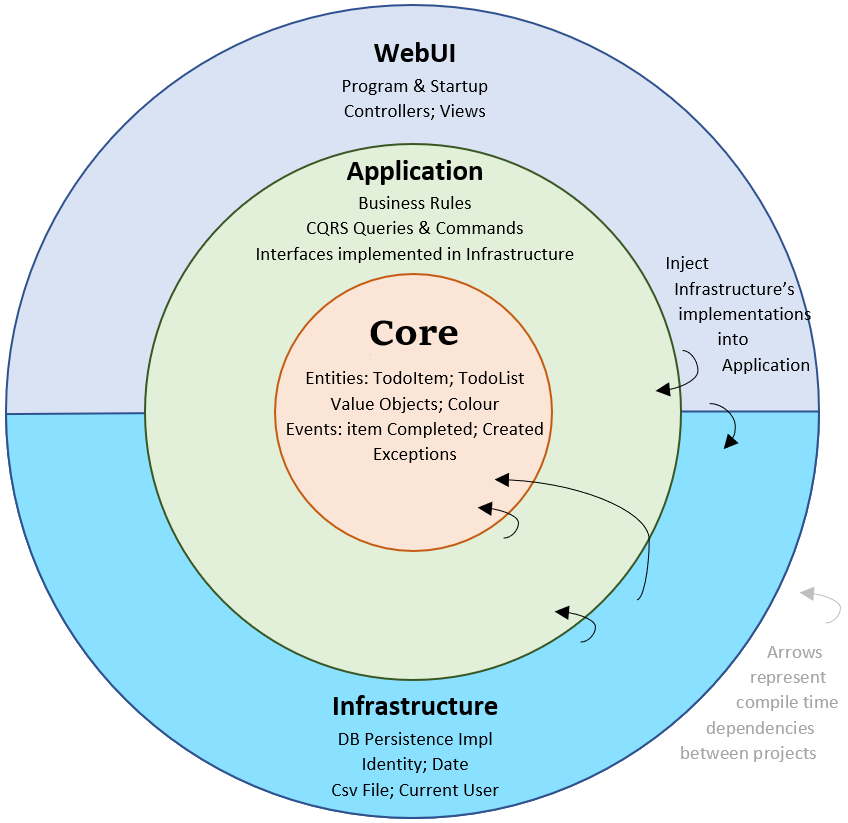
\includegraphics[width=0.6\textwidth] {images/clean_architecture.png}
    \caption{Clean Architecture}
    \label{fig:clean_architecture}
\end{figure}

\newpage

\subsection{Stratul de bază}

Stratul de bază, sau central, reprezintă nucleul aplicației și conține regulile de business și logică aplicației. Acesta este independent față de restul straturilor, neavând dependințe către niciun dintre ele. Acestă independența permite testarea și refacerea acestuia independent de restul aplicației. Acesta este împărțit în trei părți importante: Entities, Use Cases și Interfaces.

\begin{itemize}
    \item \textbf{Entities} - reprezintă obiectele de bază ale aplicației, care conțin regulile de business și logică aplicației. În acest caz, printre entități se numără: User, Pet, Appointment, etc. și conțin doar datele și metodele necesare pentru a le manipula, fără a avea niciun fel de dependință către alte componente ale aplicației.
    \item \textbf{Use Cases} - reprezintă regulile de business ale aplicației, de exemplu: adăugarea unui nou utilizator, inregistrarea unui animal de companie, realizarea unei programări, etc. Acestea sunt independente de orice altă parte a aplicației, ceea ce înseamnă că pot fi testate fără a fi nevoie de alte componente. 
    \item \textbf{Interfaces} - reprezintă interfețele de comunicare cu celelalte straturi ale aplicației. Aici se regăsesc interfețele pentru baza de date, serviciile web, etc.
    
\end{itemize}

\subsection{Stratul de aplicație}

Stratul de aplicație în arhitectura "Clean Architecture" reprezintă puntea între interfața utilizatorului și logica de afaceri din Stratul de paza. Gestionează fluxului de date și de interacțiunea între componentele UI (User Interface) și componentele din Core. 

Nivelul de aplicație conține următoarele componente: 

\begin{itemize}
    \item \textbf{Commands} - Comenzile sunrt reprezentate de cereri sau acțiuni specifice pe care un utilizator le poate efectua in intermediul aplicației. Aceastea includ acțiuni precum crearea obiectelor, actualizarea datelor sau ștergerea acestora. Comenzile sunt de obicei reprezentate de structuri de date care conțin informațiile necesare pentru a efectua acțiunea dorită.
    \item \textbf{Handlers} Handler-ii, sau gestionatorii, sunt componente responsabile pentru acceptarea și gestionarea comenzilor primite, ocupându-se de execuția logicii asociate cu acea comandă. Handler-ul primește comanda, extrage datele necesare și apelează funcțiile corespunzătoare din stratul de bază pentru a efectua operația necesară. Ele pot interacționa cu alte servicii din stratul curent, cum ar fi mappers sau responses, pentru a efectua acțiunile dorite și a returna rezultatele corespunzătoare.
    \item \textbf{Queries} - interogările reprezintă in general cereri de informații din partea utilizatorului. Acestea implica de obicei extragerea datelor din baza de date, prelucrarea lor intr-un anumit mod și returnarea acestora către utilizator. Spre deosebire de comenzi care modifică starea sistemului, interogările au doar rolul de a returna informații într-o formă cerută.
    \item \textbf{Mappers} - mapperele sunt componente care se ocupă de transformarea datelor in formatul necesar. Acestea sunt folosite pentru a transforma obiectele primite de la utilizator in obiecte din stratul de bază, sau pentru a transforma obiectele din stratul de bază în obiecte care pot fi trimise către utilizator, în funcție de caz.
    
    \newpage

    \item \textbf{Responses} - răspunsurile sunt entități asemănătoare celor din stratul de bază, fiind formate însă doar variabile. Rolul acestora este de a returna datele cerute de utilizator, după ce au fost prelucrate de către handler, dar într-un format sigur. Returnarea unui obiect din stratul de bază ar putea expune către exterior date sensibile, cum ar fi parolele, id-uri, sau ar putea expune detalii despre implementarea internă a aplicației.
\end{itemize}

\subsection{Stratul de infrastructură}

Stratul de infrastructură oferă implementarea concretă a interfețelor definite ulterior în stratul de bază. Aici sunt incluse componentele care îndeplinesc accesul la baza de date, serviciile de comunicare externă, sistemul de fișiere și alte resurse externe. Stratul conține următoarele componente:


\begin{itemize}
    \item \textbf{Repositories} - reprezintă implementarea detaliată a interfețelor din stratul de bază și sunt responsabile pentru accesul la baza de date. Ele sunt folosite de handleri pentru a introduce, extrage, modifica sau șterge informațiile din baza de date.
    \item \textbf{Services} - serviciile sunt componente care 
    asigură comunicarea cu alte servicii externe, precum servicii web sau servicii de stocare în cloud. Acestea sunt folosite de handleri pentru a efectua operațiunile necesare.
\end{itemize}

\subsection{Stratul de interfață}

Stratul de interfață reprezintă este responsabil pentru interacțiunea cu utilizatorul. Aici se gasesc componentele pentru interfața cu utilizatorul (interfață web, API, etc.). Acest strat are rolul de a prelua datele de la utilizator, de a le trimite mai departe către handleri si de a returna datele cerute. Principala componentă a acestui strat este API-ul, care este folosit de aplicația mobilă pentru a comunica cu serverul.

\begin{itemize}
    \item \textbf{Controllers} - Controller-ii din API-uri acționează ca intermediari între partea de prezentare, interfața utilizatorului, și restul aplicației. Aceștea primesc cereri HTTP de la clienți pe care le trimit către handlerii din stratul de applicatie. Aici cererea este îndeplinită și ulterior handlerii returnează datele către controller care, la rândul sau, le trimite mai departe către client.
\end{itemize}

\newpage


\section{Arhitectura aplicației mobile}



\section{Arhitectura bazei de date}


Pentru baza de date, am ales să folosesc SQL Server, un sistem de management al bazelor de date relaționale. Dezvoltat de Microsoft, SQL Server oferă o bază solidă pentru stocarea datelor într-un mod structurat și eficient. Fiind un sistem relațional, acesta permite definirea și gestionarea tabelelor și relațiilor dintre ele, facilitând organizarea datelor într-un format coerent.

SQL Server acceptă o varietate de tipuri de date, cum ar fi șiruri, numere, date și ore care vă permit să gestionați și manipulați aceste informații folosind funcții și operațiuni specifice. De asemenea, oferă suport pentru funcții și proceduri stocate, permițându-vă să creați o logică personalizată reutilizabilă în baza de date.

Un aspect cheie al SQL Server este capacitatea sa de a lucra cu date spațiale. Aceasta înseamnă că puteți stoca și manipula informații geospațiale, cum ar fi coordonatele geografice și poligoane. Această caracteristică este utilă în aplicații precum cea prezentată care necesită manipularea datelor spațiale pentru a oferi funcționalități precum navigarea sau afișarea unei locații pe hartă.

\subsection{Avantajele aduse de Sql Server}

\begin{itemize}
    \item \textbf{Performanța\footnote{Itzik Ben-Gan, Adam Machanic, Dejan Sarka, Kevin Farlee, Performance Tuning
    and Optimization in SQL Server, Microsoft Press}} - SQL Server este recunoscut pentru capacitatea sa de gestiona cantități mari de date si performanța sa ridicată. Oferă suport pentru indexarea datelor, care permite acces rapidă la date, și optimizarea interogărilor. De asemenea, oferă suport pentru funcții și proceduri stocate, care permit crearea de funcționalități complexe care pot fi apoi reutilizate în cadrul aplicației.
    \item \textbf{Securitatea} - acesta pune la dispozitie o mulțime de funcționalități de securitate robuste pentru protejarea datele stocate în baza de date. Aici sunt incluse autorizarea, criptarea și auditarea, care asigură integritatea și confidențialitate informaților.
    
    \newpage

    \item \textbf{Integrare cu mediul .NET} - ambele produse fiind dezoltate de Microsoft, SQL Server si .NET sunt compatibile și se integrează perfect. Acest lucru facilitează interacțiunea dintre serverul ASP.NET și baza de date, permițându-ne să accesăm și să manipulăm date într-un mod simplu și eficient.
    \item \textbf{Măsuri de siguranță} - SQL Server oferă o serie de mecanisme utile pentru a asigura integritatea datelor în cazul unor evenimente neprevăzute. Funcții precum tranzacții, jurnale de tranzacții și backup-uri periodice ajută la protejarea datelor și la recuperarea lor în cazul unor erori de sistem sau erori umane.
\end{itemize}

\subsection{Diagrama bazei de date}

\begin{figure}[ht]
    \centering
    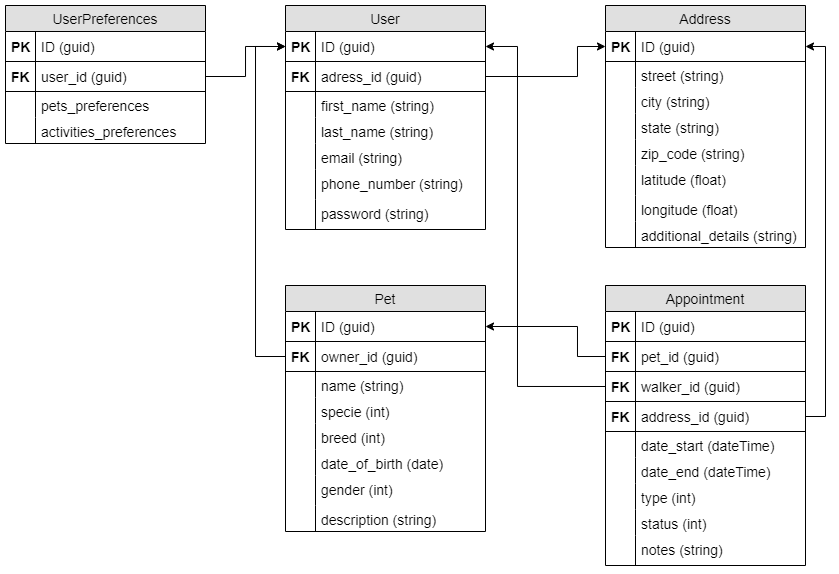
\includegraphics[width=1\textwidth] {images/database.png}
    \caption{Diagrama bazei de date}
    \label{fig:database}
\end{figure}